\documentclass[preprint,12pt]{elsarticle}

\usepackage[utf8]{inputenc}
\usepackage[T1]{fontenc}
\usepackage{lmodern}
\usepackage{booktabs}
\usepackage{tabularx}
\usepackage{array}
\usepackage{enumitem}
\usepackage{listings}
\usepackage{xcolor}
\usepackage{tikz}
\usepackage{hyperref}
\usetikzlibrary{arrows.meta,positioning,fit}

\hypersetup{
  colorlinks=true,
  linkcolor=black,
  citecolor=black,
  urlcolor=black
}

\lstdefinestyle{osl}{
  basicstyle=\ttfamily\small,
  breaklines=true,
  columns=fullflexible,
  frame=single,
  keepspaces=true
}

\journal{Advanced Engineering Informatics}

\begin{document}

\begin{frontmatter}

\title{From Situated Field Notes to Operator Strategy Models: Eliciting Manufacturing Knowledge for Digital Twin Development}

\author[hiost]{Martin Arthur Andersen\corref{cor1}}
\ead{nks.rap@gmail.com}
\cortext[cor1]{Corresponding author.}

\author[hiost]{Co-author Name}

\address[hiost]{Østfold University College, Halden, Norway}

\begin{abstract}
Digital Twin development in manufacturing depends on operational knowledge that is often unavailable in machine documentation, sensor streams, or formal process descriptions alone. Operators interpret sounds, vibrations, alarms, tooling behaviour, workarounds, and exceptions as part of situated practice, yet these interpretations are rarely transformed into traceable and model-ready artefacts before Digital Twin design begins. This paper presents Notebook-to-OSL, a hybrid elicitation-and-transformation method for capturing operator strategies during apprenticeship-like CNC operator training and preparing them for formalisation. The method combines contextual inquiry, situated learning, cognitive task analysis, requirements engineering, and model-based systems engineering. In the proposed workflow, a researcher captures low-friction digital field notes during training, then selects, annotates, clarifies, validates, and transforms them into operator-strategy fragments. The paper contributes a literature-grounded workflow, an annotation schema covering cues, context, interpretation, action, rationale, exception, uncertainty, risk, responsibility, traceability, and validation needs, and a pilot-oriented evaluation protocol for assessing whether fragments become model-ready candidates. The contribution is positioned as an intermediate knowledge layer between situated operator practice and formal Digital Twin artefacts such as requirements, decision-support rules, SysML elements, knowledge-graph structures, or future Operator Strategy Language constructs. The paper argues that human-in-the-loop Digital Twins require not only connected data and models, but also explicit methods for preserving the situated reasoning that makes operator support meaningful.
\end{abstract}

\begin{keyword}
Digital Twin \sep Operator strategy \sep Situated elicitation \sep Contextual inquiry \sep Cognitive task analysis \sep Requirements elicitation \sep Model-based systems engineering \sep Human-in-the-loop systems
\end{keyword}

\end{frontmatter}

\section{Introduction}
\label{sec:introduction}

Digital Twins are increasingly presented as foundations for monitoring, simulation, prediction, optimisation, and decision support in manufacturing. Foundational and review literature emphasises virtual--physical linkage, lifecycle information, data integration, simulation, and synchronisation \cite{grieves2017digital,kritzinger2018digital,fuller2020digital,negri2017review,semeraro2021digital}. These perspectives are necessary, but they explain Digital Twin development mainly through architectures, data flows, and model integration. They say less about how operator knowledge is elicited, interpreted, validated, and represented before formal modelling begins.

This omission matters for human-\allowbreak in-\allowbreak the-\allowbreak loop Digital Twins. Operators do not only use dashboards or respond to alarms. They interpret machine behaviour through situated cues such as sound, vibration, rhythm, surface finish, tool behaviour, alarm combinations, and deviations from expected response. Their actions depend on context, uncertainty, production risk, escalation paths, and trust in the available evidence. Human-centred Digital Twin research has therefore begun to ask where humans fit in the Digital Twin loop and how collaboration, responsibility, and trust should be distributed between human actors and digital systems \cite{agrawal2023humans,longo2022ubiquitous,lee2004trust,parasuraman2000levels}. A practical gap remains between recognising that operator knowledge matters and establishing what situated elicitation captures, how researcher interpretation changes through operator review, and whether the validated knowledge can be represented coherently for later engineering use.

We address that gap through the notion of an \emph{operator-strategy fragment}. An operator-strategy fragment is an intermediate knowledge object that relates an operational observation to its context, interpretation, possible responses, rationale, uncertainty, risk, responsibility, and validation state. It is more structured than a raw field note, but less formal than an executable rule or complete Digital Twin model. This intermediate status is important because premature formalisation can erase precisely the contextual judgement that makes operator knowledge useful.

This paper presents \emph{Notebook-to-OSL}. The method is designed for apprenticeship-like situations where a researcher or engineer stands beside an operator and is trained in the work process. During the training session, the researcher captures low-friction digital field notes rather than forcing each observation into a schema. A short post-session interview over the same task scope provides a comparison source. The researcher then annotates the captured material, records an initial interpretation, reviews it with the operator, and transforms validated fragments into candidate formal representations. OSL, short for Operator Strategy Language, is treated as one downstream target. The contribution is not the complete language or a runtime Digital Twin; it is a study design and transformation method that makes the path from situated explanation to formal representation inspectable.

The method is grounded in five bodies of literature. Contextual inquiry supports learning from real work in context and treating interpretation as a collaborative activity \cite{beyer1995apprenticing,beyer1997contextual}. Situated learning and cognitive apprenticeship justify the training situation as an elicitation setting in which expert reasoning becomes visible through demonstration, coaching, articulation, and reflection \cite{lave1991situated,collins1989cognitive}. Cognitive task analysis supports the focus on cues, difficult decisions, hidden judgments, alternatives, and expert--novice differences \cite{crandall2006workingminds,klein1989critical,stanik2021acta}. Requirements engineering and systems engineering provide traceability, rationale, risk, source, status, and validation principles \cite{vanlamsweerde2009requirements,sebokStakeholder,sebokRequirements}. Finally, MBSE and semantic Digital Twin research motivate the assessment of whether validated fragments can support formal representations such as SysML v2, requirements, knowledge graphs, or OSL constructs \cite{omgSysml2024,karabulut2023ontologies,listl2024knowledge,braun2022graph}.

The paper addresses three research questions:

\begin{description}[leftmargin=2.4cm,style=nextline]
    \item[RQ1] How does situated CNC operator training differ from a conventional post-session interview in the operator-strategy knowledge it elicits?
    \item[RQ2] How does operator validation change the researcher's interpretation of captured notes?
    \item[RQ3] To what extent can validated operator-strategy fragments be transformed into traceable, semantically coherent OSL representations, and what gaps remain?
\end{description}

The paper is organised around these questions. For RQ1, it defines a comparative elicitation design that separates material captured during situated training from material elicited in a short post-session interview. For RQ2, it defines a traceable interpretation and validation workflow that records whether fragments are accepted, corrected, narrowed, rejected, or marked sensitive. For RQ3, it defines a model-readiness assessment that tests whether validated fragments can be transformed without losing context, uncertainty, alternatives, provenance, or unresolved knowledge gaps. The annotation schema and illustrative CNC transformation support these three analyses rather than constituting separate contributions detached from the research questions.

The remainder of the paper follows the same structure. Section~\ref{sec:background} establishes the theoretical basis for the three questions. Section~\ref{sec:research-design} maps each question to its data, comparison, and analysis. Section~\ref{sec:method} defines the situated capture, interview, interpretation, validation, and transformation workflow. Section~\ref{sec:schema} specifies the information required to conduct the analyses. Section~\ref{sec:case} illustrates the trace from raw note to formal candidate. Section~\ref{sec:discussion} discusses the contribution and evaluation logic question by question. Section~\ref{sec:conclusion} summarises what the proposed study can establish and what requires empirical application.

\section{Background and related work}
\label{sec:background}

\subsection{Digital Twins in manufacturing}

Digital Twin research in manufacturing has developed around virtual representations of physical assets, physical--digital connectivity, lifecycle data, simulation, monitoring, and synchronisation \cite{grieves2017digital,kritzinger2018digital,tao2018digital,fuller2020digital}. Reviews show that manufacturing remains a central Digital Twin domain, with recurring attention to production systems, predictive maintenance, optimisation, cyber-physical integration, and interoperability \cite{negri2017review,semeraro2021digital}. These works provide the technical baseline for the present paper: a Digital Twin is not merely a static model, but a connected digital representation that can support understanding, prediction, and decision-making.

However, the literature is less mature on the front-end problem of how the knowledge needed for a useful Digital Twin is elicited from work practice. Manufacturing Digital Twin papers often focus on asset data, simulation models, control architectures, or integration levels. Human knowledge is frequently assumed to enter through requirements, domain expertise, dashboard design, or validation, but the transformation from situated operator explanation to structured Digital Twin knowledge is rarely the main object of study.

\subsection{Human-in-the-loop and human-centred Digital Twins}

Human-in-the-loop Digital Twin research argues that Digital Twins should not be understood as fully autonomous replacements for human expertise. Instead, they should distribute observation, interpretation, decision-making, and responsibility between digital systems and human actors. Work on human roles in Digital Twins highlights that decisions about automation, human oversight, trust, and responsibility are often under-specified \cite{agrawal2023humans,parasuraman2000levels,lee2004trust}. Human-centred smart-factory research similarly emphasises that shop-floor workers remain central to knowledge creation, interpretation, and operational adaptation \cite{longo2022ubiquitous}.

For Notebook-to-OSL, this literature justifies treating operators as knowledge-bearing participants in Digital Twin development rather than only as end users. It also shows why the output of elicitation must preserve responsibility, escalation, and validation needs. A recommendation or alarm in a Digital Twin is only useful if the system also represents when an operator should trust it, when it should be checked, and who is responsible for acting.

\subsection{Operator knowledge, situation awareness, and expert judgement}

The knowledge used by operators is often partly tacit. Polanyi's account of tacit knowledge is commonly summarised by the idea that people can know more than they can explicitly tell \cite{polanyi1966tacit}. In manufacturing, this is visible when operators recognise abnormal behaviour through experience-based cues that are difficult to specify in advance. Such cues may include sound, vibration, smell, timing, tool marks, alarm combinations, or the relation between machine response and operation context.

Operator decision-making also depends on situation awareness and control context. Endsley describes situation awareness in terms of perceiving elements in the environment, comprehending their meaning, and projecting future status \cite{endsley1995situation}. Rasmussen's distinction between skill-, rule-, and knowledge-based behaviour shows that action in technical systems cannot be reduced to isolated commands \cite{rasmussen1983skills}. Together, these perspectives imply that a Digital Twin should not only capture that an operator acts, but also what the operator noticed, how the cue was interpreted, and why the action was judged appropriate.

\subsection{Situated learning, cognitive apprenticeship, and contextual inquiry}

Situated learning theory argues that learning is embedded in social and material practice rather than detached from context \cite{lave1991situated}. Cognitive apprenticeship makes a related argument in design terms: expert reasoning can be made visible through modelling, coaching, scaffolding, articulation, reflection, and exploration \cite{collins1989cognitive}. This is directly relevant to the proposed training situation. When an operator teaches a researcher how a CNC process is understood and handled, the operator is not only transmitting information; they are demonstrating how expertise is enacted in context.

Contextual inquiry provides a more operational method base. Its classic orientation is to study work where it happens, in partnership with the practitioner, and to treat interpretations as things that should be checked rather than silently inferred \cite{beyer1995apprenticing,beyer1997contextual}. Contextual design also shows that field observations can be transformed into structured work models. Notebook-to-OSL adopts this logic but narrows the target: rather than modelling the whole work system or immediately designing a user interface, it captures operator-strategy fragments that can later inform Digital Twin artefacts.

\subsection{Cognitive task analysis and hidden decision knowledge}

Contextual inquiry is strong on work setting, artefacts, flow, and interpretation, but it is less specific about hidden cognitive demands. Cognitive task analysis (CTA) and the critical decision method focus more directly on expertise, decision points, cues, anomalies, difficult judgments, and expert--novice differences \cite{crandall2006workingminds,klein1989critical}. ACTA-based work has also shown how CTA can be customised for design and requirements-oriented projects, where expert cognition must be elicited and converted into design-relevant outputs \cite{stanik2021acta}.

Notebook-to-OSL uses CTA as a clarification layer. During live training, the researcher should avoid turning the situation into a formal interview. After the session, however, selected notes can be probed with CTA-inspired questions: What first indicated that this was abnormal? What would a novice miss? What else could this cue mean? When would the action be wrong? When should the situation be escalated? These questions help recover cognitive structure without overloading the live training session.

\subsection{Requirements engineering, MBSE, and model-ready transformation}

Requirements engineering and systems engineering add the rigor needed to turn field material into engineering artefacts. Requirements work distinguishes stakeholder statements, needs, rationale, risks, constraints, verification criteria, and formal specifications \cite{vanlamsweerde2009requirements}. SEBoK guidance similarly emphasises stakeholder identification, source traceability, rationale, risks, status, ownership, and transformation from stakeholder needs to system requirements \cite{sebokStakeholder,sebokRequirements}. These principles justify why the Notebook-to-OSL schema includes fields such as source, rationale, uncertainty, risk, validation need, responsibility, and status.

The downstream modelling literature is also relevant. EARS provides lightweight controlled natural-language patterns for transforming messy requirements statements into more consistent requirement-like structures \cite{mavin2009ears}. SysML v2 provides a formal MBSE target for requirements, structure, behaviour, analysis, and verification artefacts \cite{omgSysml2024}. Semantic Digital Twin work using ontologies and knowledge graphs shows that Digital Twin knowledge is increasingly represented as reusable and interoperable structures rather than isolated documents \cite{karabulut2023ontologies,listl2024knowledge,braun2022graph}. These works motivate the term \emph{model-ready}: the fragment does not need to be fully formal, but it must contain enough structure to support later mapping to requirements, OSL, SysML v2, rules, or semantic models.

\subsection{Synthesis and research gap}

The literature provides strong components but not the complete method needed here. Contextual inquiry and situated learning support learning from real work in context. CTA supports probing cues and expert decisions. Requirements engineering and MBSE support traceability, rationale, risk, and transformation. Semantic Digital Twin literature supports model-ready knowledge structures. What remains underdeveloped is the bridge between these elements: a practical workflow for converting situated operator-training notes into traceable, uncertainty-aware, validated, model-ready operator-strategy fragments for human-in-the-loop Digital Twin development. Notebook-to-OSL is proposed as that bridge.

\section{Research design and scope}
\label{sec:research-design}

This paper is written as a method paper with an explicit empirical evaluation design. Its purpose is to define and justify a repeatable workflow for comparing situated and interview-based elicitation, tracing changes introduced by operator validation, and assessing whether validated fragments can be transformed into semantically coherent OSL representations. The method is intended for early-stage manufacturing projects where operator reasoning is important, but where Digital Twin requirements, models, and decision-support logic have not yet been formalised.

\subsection{Methodological position}

Notebook-to-OSL is a hybrid method rather than a new method family. It combines three layers. The elicitation layer is contextual and apprenticeship-based, with a conventional post-session interview used as a comparison source. The interpretation layer is cognitive-task-analysis-inspired: selected notes are examined for cues, difficult decisions, alternatives, expert--novice differences, exceptions, and escalation logic. The transformation layer is requirements- and MBSE-oriented: validated fragments are given traceability, status, rationale, and an explicit path toward formal representation.

Table~\ref{tab:method-family-comparison} summarises how the main literature streams contribute to the method.

\begin{table}[htbp]
\centering
\caption{Literature streams used to ground Notebook-to-OSL.}
\label{tab:method-family-comparison}
\begin{tabularx}{\textwidth}{p{0.25\textwidth}p{0.33\textwidth}X}
\toprule
Method family & Contribution to Notebook-to-OSL & Limitation if used alone \\
\midrule
Contextual inquiry and contextual design & Captures work in context, preserves operator phrasing, artefacts, flow, and interpretation checks \cite{beyer1995apprenticing,beyer1997contextual}. & Does not by itself establish what situated elicitation adds relative to a conventional interview. \\
Situated learning and cognitive apprenticeship & Justifies training as an elicitation setting where expert reasoning is demonstrated, coached, articulated, and reflected upon \cite{lave1991situated,collins1989cognitive}. & Provides theoretical framing but not a complete comparison or transformation protocol. \\
Cognitive task analysis & Surfaces cues, difficult judgments, expert--novice differences, anomalies, alternatives, and decision points \cite{crandall2006workingminds,klein1989critical,stanik2021acta}. & Can be intrusive during live work if applied as a full interview protocol. \\
Requirements engineering and SEBoK & Adds traceability, source, rationale, risk, status, ownership, and validation principles \cite{vanlamsweerde2009requirements,sebokStakeholder,sebokRequirements}. & Operates after stakeholder knowledge has been elicited and may conceal interpretation changes if provenance is weak. \\
MBSE and semantic DT modelling & Provides downstream targets such as SysML v2, controlled requirements, rules, and knowledge graphs \cite{mavin2009ears,omgSysml2024,karabulut2023ontologies,listl2024knowledge}. & Can over-formalise knowledge before it is reviewed and semantically qualified. \\
\bottomrule
\end{tabularx}
\end{table}

\subsection{Research-question alignment}

The three research questions define the evidence that the study must collect and the claims it may make. Table~\ref{tab:rq-alignment} maps each question to its data and analysis.

\begin{table}[htbp]
\centering
\caption{Alignment between research questions, evidence, and analysis.}
\label{tab:rq-alignment}
\begin{tabularx}{\textwidth}{p{0.09\textwidth}p{0.30\textwidth}p{0.28\textwidth}X}
\toprule
RQ & Required evidence & Analysis & Permitted conclusion \\
\midrule
RQ1 & Separate situated-training notes and post-session interview material covering the same task scope. & Compare which observations, contexts, interpretations, actions, exceptions, risks, and uncertainties occur in each source. & Whether and how the two elicitation settings produce different operator-strategy knowledge in the studied case. \\
RQ2 & Initial researcher annotations and operator-review records for the same fragments. & Trace accepted, corrected, narrowed, rejected, and sensitive interpretations and characterise the changes. & How operator review changes the researcher's interpretation and which categories are most vulnerable to misinterpretation. \\
RQ3 & Validated fragments, candidate OSL representations, transformation decisions, and unresolved gaps. & Assess traceability, semantic coherence, information loss, explicit incompleteness, and unsupported mappings. & Which validated fragments can be represented coherently, which remain incomplete, and where the representation requires refinement. \\
\bottomrule
\end{tabularx}
\end{table}

This alignment prevents the paper from treating the workflow, schema, and OSL example as independent contributions. They are research instruments used to answer the three questions.

\subsection{Design requirements}

The workflow should satisfy six requirements:

\begin{enumerate}[label=R\arabic*.]
    \item \textbf{Low friction during training.} The researcher must capture notes without interrupting the operator's explanation or the flow of the training situation.
    \item \textbf{Comparable sources.} Situated notes and post-session interview material must cover the same task scope and remain distinguishable during analysis.
    \item \textbf{Traceable interpretation.} Each structured fragment must remain linked to its raw source, the researcher's initial interpretation, operator-review outcome, and downstream representation.
    \item \textbf{Preservation of uncertainty.} The method must not force uncertain, context-dependent, alternative, or disputed observations into overly precise rules.
    \item \textbf{Validation before formalisation.} Operator or domain-expert review must occur before a fragment is treated as model-ready.
    \item \textbf{Assessable model-readiness.} The transformation must expose whether context, interpretation, response logic, uncertainty, provenance, and unresolved gaps can be represented coherently rather than merely producing syntactically plausible output.
\end{enumerate}

\subsection{Unit of analysis}

The primary unit of analysis is the \emph{operator-strategy fragment}. A fragment is derived from one or more raw notes or interview statements and relates an operational observation to context, interpretation, possible responses, rationale, exception, uncertainty, risk, responsibility, and validation state. The analysis also preserves the source-level distinction needed for RQ1, the version history needed for RQ2, and the transformation record needed for RQ3.

\subsection{Pilot study protocol}

A full empirical version of this paper should evaluate the method through a small but auditable pilot. The pilot should not aim to prove that a complete Digital Twin improves production performance. It should test the comparative, interpretive, and representational questions defined above.

The recommended pilot protocol is:

\begin{enumerate}
    \item Define one narrow task scope, such as one CNC monitoring task, recurring abnormality, or setup/inspection episode.
    \item Agree on consent and confidentiality boundaries, including what may be written, photographed, stored, anonymised, or excluded.
    \item Conduct a situated training session where the operator teaches the researcher in the real or simulated work setting.
    \item Capture low-friction digital field notes with identifiers, timestamps, raw text, setting, and optional task phase.
    \item Conduct a short post-session interview covering the same task scope without showing the situated notes as prompts.
    \item Keep situated and interview material separate, then code both with the same initial categories to answer RQ1.
    \item Create an initial researcher annotation for selected fragments and preserve that version.
    \item Apply CTA-style clarification where cues, alternatives, thresholds, or action logic remain ambiguous.
    \item Review the annotations with the operator and record each acceptance, correction, narrowing, rejection, or sensitivity decision to answer RQ2.
    \item Transform validated fragments into candidate OSL representations and record successful mappings, information loss, explicit gaps, and unsupported mappings to answer RQ3.
\end{enumerate}

\subsection{Empirical material and metrics}

Table~\ref{tab:empirical-material} summarises the minimum material needed for the pilot.

\begin{table}[htbp]
\centering
\caption{Minimum empirical material and its role in the research questions.}
\label{tab:empirical-material}
\begin{tabularx}{\textwidth}{p{0.27\textwidth}p{0.12\textwidth}X}
\toprule
Material & RQ & Purpose \\
\midrule
Situated training note log & RQ1 & Preserve knowledge captured while the operator demonstrates and explains work in context. \\
Post-session interview record & RQ1 & Provide a conventional elicitation comparison over the same task scope. \\
Initial annotation set & RQ2 & Preserve the researcher's interpretation before operator review. \\
Clarification and operator-review log & RQ2 & Record why interpretations were accepted, corrected, narrowed, rejected, or restricted. \\
Validated fragment set & RQ2--RQ3 & Establish the reviewed knowledge eligible for formal transformation. \\
Candidate OSL representations and mapping log & RQ3 & Show which semantic structures can be represented and which gaps remain. \\
Reflection log & All & Document researcher bias, missed context, methodological deviations, and confidentiality decisions. \\
\bottomrule
\end{tabularx}
\end{table}

For RQ1, the analysis should report source-exclusive and shared knowledge elements rather than only total note counts. For RQ2, it should report the number and type of interpretation changes and provide qualitative examples of consequential corrections. For RQ3, it should report the proportion of validated fragments that can be represented with traceability and semantic coherence, the proportion that remain explicitly incomplete, and the recurring reasons why transformation fails or loses information. These measures are descriptive and case-bounded; they do not establish general superiority, operational correctness, or safety.

\subsection{Scope and boundaries}

The paper does not claim to deliver a complete Operator Strategy Language or a complete Digital Twin. It focuses on the intermediate research problem between situated operator learning and formal modelling. RQ1 is limited to the elicitation settings studied. RQ2 evaluates interpretation change, not universal operator agreement. RQ3 evaluates representation adequacy for the validated fragments, not runtime matching, automatic recommendation, operational correctness, or safety.

The tool is treated as a research instrument that supports capture, versioning, review, and transformation. OSL is treated as the formal target needed to examine RQ3. Neither the tool nor the language is validated merely because the workflow can produce an artefact.

\section{Notebook-to-OSL method}
\label{sec:method}

Notebook-to-OSL is a workflow for comparing situated and interview-based elicitation, tracing interpretation changes through operator review, and assessing formal transformation. The method is grounded in the alignment in Section~\ref{sec:research-design}: contextual inquiry and situated learning define the situated capture setting for RQ1; a bounded post-session interview provides the comparison source; cognitive task analysis and operator review define the interpretation checks for RQ2; and requirements engineering, MBSE, and OSL define traceability and model-readiness for RQ3. Figure~\ref{fig:notebook-to-osl-workflow} summarises the core transformation path.

\begin{figure}[htbp]
    \centering
    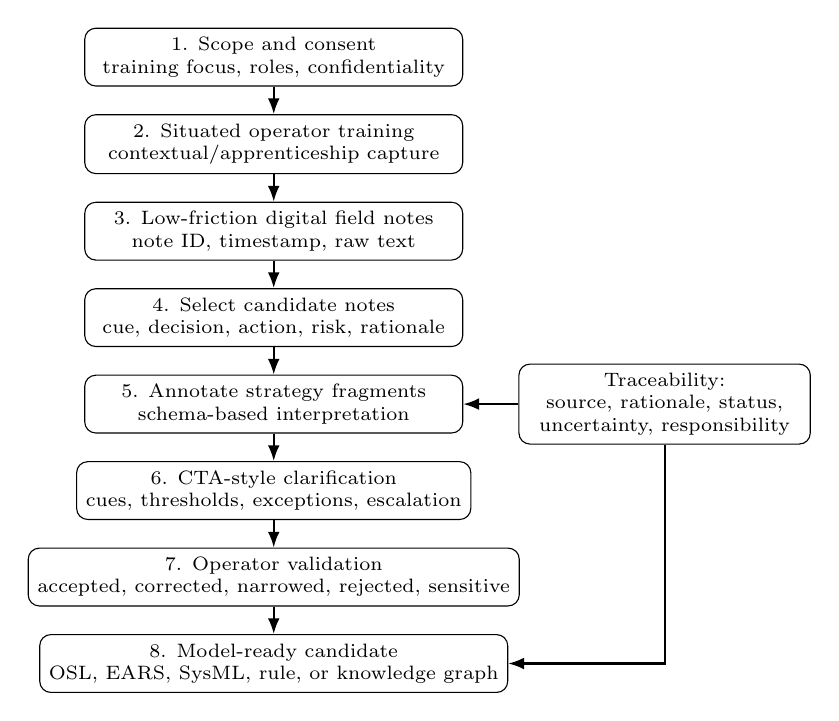
\begin{tikzpicture}[
  node distance=3.5mm,
  box/.style={draw, rounded corners, align=center, minimum width=48mm, minimum height=6mm, font=\scriptsize},
  side/.style={draw, rounded corners, align=center, minimum width=37mm, minimum height=6mm, font=\scriptsize},
  arrow/.style={-{Latex[length=2mm]}, thick}
]

\node[box] (scope) {1. Scope and consent\\training focus, roles, confidentiality};
\node[box, below=of scope] (training) {2. Situated operator training\\contextual/apprenticeship capture};
\node[box, below=of training] (raw) {3. Low-friction digital field notes\\note ID, timestamp, raw text};
\node[box, below=of raw] (select) {4. Select candidate notes\\cue, decision, action, risk, rationale};
\node[box, below=of select] (annotate) {5. Annotate strategy fragments\\schema-based interpretation};
\node[box, below=of annotate] (clarify) {6. CTA-style clarification\\cues, thresholds, exceptions, escalation};
\node[box, below=of clarify] (validate) {7. Operator validation\\accepted, corrected, narrowed, rejected, sensitive};
\node[box, below=of validate] (model) {8. Model-ready candidate\\OSL, EARS, SysML, rule, or knowledge graph};

\draw[arrow] (scope) -- (training);
\draw[arrow] (training) -- (raw);
\draw[arrow] (raw) -- (select);
\draw[arrow] (select) -- (annotate);
\draw[arrow] (annotate) -- (clarify);
\draw[arrow] (clarify) -- (validate);
\draw[arrow] (validate) -- (model);

\node[side, right=7mm of annotate] (trace) {Traceability:\\source, rationale, status,\\uncertainty, responsibility};
\draw[arrow] (trace) -- (annotate);
\draw[arrow] (trace) |- (model);

\end{tikzpicture}

    \caption{Core Notebook-to-OSL transformation path from situated capture to validated model-ready candidate. The RQ1 comparison additionally preserves a separate post-session interview source.}
    \label{fig:notebook-to-osl-workflow}
\end{figure}

The method is organised into nine phases. Table~\ref{tab:workflow} identifies the output and the research question supported by each phase.

\begin{table}[htbp]
\centering
\caption{Notebook-to-OSL workflow phases, outputs, and research-question roles.}
\label{tab:workflow}
\begin{tabularx}{\textwidth}{p{0.25\textwidth}p{0.13\textwidth}X}
\toprule
Phase & RQ & Output \\
\midrule
1. Scope and consent & All & Task focus, stakeholder roles, and confidentiality boundary. \\
2. Situated training & RQ1 & Context-bound operator explanations, demonstrations, and observations. \\
3. Low-friction note capture & RQ1 & Timestamped field notes preserving raw phrasing and task context. \\
4. Post-session interview & RQ1 & Separate interview material covering the same task scope. \\
5. Source comparison and selection & RQ1--RQ2 & Shared and source-exclusive knowledge elements plus candidate fragments. \\
6. Initial annotation & RQ2 & Versioned researcher interpretations linked to their sources. \\
7. CTA-style clarification & RQ2 & Clarified cues, alternatives, thresholds, exceptions, and escalation logic. \\
8. Operator validation & RQ2 & Accepted, corrected, narrowed, rejected, or sensitive fragments. \\
9. OSL transformation assessment & RQ3 & Traceable candidate representations, explicit gaps, and failed mappings. \\
\bottomrule
\end{tabularx}
\end{table}

\subsection{Phase 1: Define scope and consent}

Before data collection, the researcher defines one narrow task scope. The scope may be one machine, operation type, monitoring task, recurring abnormality, quality concern, or decision point. The same scope must be used for situated training and the post-session interview so that RQ1 compares elicitation settings rather than unrelated topics. Confidentiality boundaries should define what may be written, photographed, stored, anonymised, or excluded.

\subsection{Phase 2: Participate in situated training}

During the session, the operator trains the researcher in the work process. The researcher prioritises following the explanation, observing artefacts, and understanding task flow. Clarification questions should remain short and context-sensitive. Questions such as ``what made that matter?'', ``how would you know this is normal?'', or ``what would make you stop?'' are preferable to abstract design questions. The value of the setting is that explanations occur while the operator points, demonstrates, responds, and corrects.

\subsection{Phase 3: Capture low-friction field notes}

The researcher writes short digital field notes during the session. The capture interface should be minimal: note identifier, timestamp, raw text, optional task phase, optional artefact reference, and save action. The researcher should not attempt to complete the full annotation schema during live work. Excessive structuring can disrupt the training and bias what is noticed.

\subsection{Phase 4: Conduct the post-session interview}

After the situated session, the researcher conducts a short conventional interview covering the same task scope. The situated notes should not be shown as prompts during the initial interview pass because doing so would collapse the two sources. The interview should ask the operator to explain relevant cues, decisions, actions, exceptions, risks, and escalation paths from memory. This phase does not assume that either source is superior; it creates the evidence needed to examine how they differ.

\subsection{Phase 5: Compare sources and select candidate fragments}

Situated notes and interview material remain separately identified. The researcher codes both with the same broad categories and records which knowledge elements are shared, situated-only, or interview-only. Candidate fragments are then selected when either source contains or implies an observation, context, interpretation, decision, response, rationale, exception, uncertainty, risk, responsibility, trust concern, or escalation path. This source comparison is the primary analysis for RQ1.

\subsection{Phase 6: Create the initial annotation}

Selected material is annotated using the schema in Section~\ref{sec:schema}. Annotation is an interpretation step, not a mechanical transcription. The initial researcher version must be preserved before clarification or operator review. If the researcher is unsure about the observation, context, interpretation, response threshold, or rationale, the fragment should be marked as uncertain or incomplete rather than silently completed. This version history provides the baseline for RQ2.

\subsection{Phase 7: Apply CTA-style clarification}

For fragments containing hidden reasoning or ambiguous response logic, the researcher applies a bounded CTA-inspired clarification step. Useful prompts include:

\begin{itemize}
    \item What first indicated that this situation was normal or abnormal?
    \item What would a novice likely miss here?
    \item What else could this observation mean?
    \item When would this interpretation be wrong?
    \item Which responses are alternatives rather than a fixed sequence?
    \item What criterion would justify selecting one response over another?
    \item Who should be contacted if the operator is uncertain?
\end{itemize}

Clarification answers remain traceable to the fragment and do not overwrite the initial interpretation.

\subsection{Phase 8: Validate with the operator or domain expert}

The operator reviews the annotated fragment. Validation should test the source interpretation, applicability context, alternatives, response logic, thresholds, risk, exception, responsibility, and confidentiality status. Each fragment is classified as \texttt{accepted}, \texttt{corrected}, \texttt{narrowed}, \texttt{rejected}, or \texttt{sensitive}. The study records both the disposition and the substantive change. These change records answer RQ2; a final accepted label alone is insufficient.

\subsection{Phase 9: Assess OSL transformation}

Only validated or explicitly bounded fragments are assessed for OSL transformation. The purpose is not merely to generate syntactically plausible output. The transformation must preserve source traceability, applicability, observations, interpretations or hypotheses, candidate and selected responses, action roles, expected consequences, uncertainty, evidence, and unresolved gaps where these are present in the source material. A fragment may therefore be classified as coherently represented, represented but explicitly incomplete, partially represented with information loss, or unsupported by the current representation. This assessment answers RQ3.

\subsection{Risk mitigation}

The method has predictable risks. The interview may be influenced by the preceding training session, live notes may be incomplete, and the researcher may over-interpret cues or impose formal categories too early. Operators may also explain differently when observed, and confidential information may appear in either source. Notebook-to-OSL mitigates these risks by preserving source separation, versioning initial interpretations, recording clarification and validation changes, marking uncertainty and sensitivity explicitly, and retaining traceability from each candidate representation back to its empirical source.

\section{Annotation schema}
\label{sec:schema}

The annotation schema is the central artefact of the method. It defines what must be preserved when a raw note is transformed into a strategy fragment. The schema is not intended to be final or universal. It is a first version that should be refined through empirical use.

\subsection{Raw note layer}

The raw note layer preserves what was captured during training. It should remain available even after annotation because later interpretation may change. Table~\ref{tab:raw-note-fields} lists the core raw note fields.

\begin{table}[htbp]
\centering
\caption{Raw note fields.}
\label{tab:raw-note-fields}
\begin{tabularx}{\textwidth}{p{0.24\textwidth}X}
\toprule
Field & Purpose \\
\midrule
\texttt{note\_id} & Stable identifier for traceability. \\
\texttt{timestamp} & Approximate time of capture. \\
\texttt{raw\_text} & Original note text. \\
\texttt{setting} & Machine, workstation, operation, or training context. \\
\texttt{speaker\_role} & Operator, researcher, engineer, maintainer, or other role. \\
\texttt{confidence\_raw} & Researcher's confidence that the note was understood correctly. \\
\bottomrule
\end{tabularx}
\end{table}

\subsection{Strategy annotation layer}

The strategy annotation layer structures the note for later modelling. Table~\ref{tab:annotation-fields} lists the proposed fields.

\begin{table}[htbp]
\centering
\caption{Strategy annotation fields.}
\label{tab:annotation-fields}
\begin{tabularx}{\textwidth}{p{0.24\textwidth}X}
\toprule
Field & Purpose \\
\midrule
\texttt{cue} & What the operator notices, such as sound, vibration, alarm, timing, tool behaviour, or visual mark. \\
\texttt{condition} & Situation in which the cue matters. \\
\texttt{interpretation} & What the cue may indicate. \\
\texttt{action} & What the operator does or considers doing. \\
\texttt{rationale} & Why the action makes sense. \\
\texttt{exception} & When the interpretation or action does not apply. \\
\texttt{uncertainty} & What is unknown, context-dependent, probabilistic, or disputed. \\
\texttt{risk} & Possible consequence if the cue is ignored or misinterpreted. \\
\texttt{validation\_need} & What must be checked with the operator or another expert. \\
\texttt{responsible\_actor} & Who acts, decides, validates, or escalates. \\
\texttt{escalation\_path} & Who is contacted if the situation cannot be resolved locally. \\
\texttt{candidate\_osl\_type} & Candidate target type, such as cue, rule, strategy, intervention, or validation gate. \\
\bottomrule
\end{tabularx}
\end{table}

\subsection{Status model}

Each note should have a status. The status prevents the repository from mixing raw, interpreted, validated, and formalised material. Table~\ref{tab:status-model} lists the proposed status values.

\begin{table}[htbp]
\centering
\caption{Status values for note transformation.}
\label{tab:status-model}
\begin{tabularx}{\textwidth}{p{0.24\textwidth}X}
\toprule
Status & Meaning \\
\midrule
\texttt{raw} & Captured during training, not yet interpreted. \\
\texttt{annotated} & Researcher has added structured fields. \\
\texttt{needs-validation} & Requires operator or domain expert review. \\
\texttt{validated} & Confirmed or corrected by operator/domain expert. \\
\texttt{formalized} & Converted into an OSL candidate or related modelling artefact. \\
\texttt{discarded} & Removed from the modelling pipeline because it is unclear, duplicate, irrelevant, or unsafe to use. \\
\bottomrule
\end{tabularx}
\end{table}

\subsection{Why uncertainty is a first-class field}

The schema treats uncertainty as a first-class field because operator strategies are often conditional. For example, a sound may indicate tool wear in one material but be normal in another. A vibration pattern may be acceptable during roughing but problematic during finishing. A Digital Twin that ignores these distinctions can create false alarms or misleading recommendations. Preserving uncertainty also supports later validation because it makes clear which parts of a fragment are confirmed and which parts remain interpretive.

\section{Illustrative CNC case}
\label{sec:case}

This section illustrates how a raw note can be transformed into an annotated strategy fragment and then into an OSL candidate. The example is intentionally generic and does not include proprietary production parameters, customer information, machine programs, or identifiable operator statements.

\subsection{Training situation}

Assume that a researcher is being trained by an experienced CNC operator. The operator explains how they monitor the cutting process during an operation. The researcher writes short notes on a laptop while standing near the machine and observing the operator's explanations. One note concerns how sound may indicate tool wear.

\subsection{Raw note}

The raw note is short and incomplete, as notes often are during situated work:

\begin{quote}
\emph{Sharper cutting sound can mean the tool is starting to wear, but not for every material. If it continues, operator checks tool before quality gets bad.}
\end{quote}

This note is not yet a requirement or rule. It contains a cue, possible interpretation, context limitation, action, and rationale. It also contains uncertainty because the cue is material-dependent.

\subsection{Annotated fragment}

Table~\ref{tab:annotated-fragment} shows a possible annotation of the note.

\begin{table}[htbp]
\centering
\caption{Example annotation of a raw training note.}
\label{tab:annotated-fragment}
\begin{tabularx}{\textwidth}{p{0.35\textwidth}X}
\toprule
Field & Value \\
\midrule
\texttt{note\_id} & N-001 \\
\texttt{raw\_text} & Sharper cutting sound can mean the tool is starting to wear, but not for every material. \\
\texttt{cue} & Sharper or brighter cutting sound. \\
\texttt{condition} & During cutting; depends on material and operation. \\
\texttt{interpretation} & Possible tool wear. \\
\texttt{action} & Continue monitoring; inspect tool if the sound persists. \\
\texttt{rationale} & Early inspection may prevent poor surface finish or tool failure. \\
\texttt{exception} & The sound may be normal for some materials or operations. \\
\texttt{uncertainty} & Cue is experience-based and not sufficient alone. \\
\texttt{risk} & Poor surface quality, scrap, or tool damage. \\
\texttt{validation\_need} & Confirm material dependency and action threshold with operator. \\
\texttt{responsible\_actor} & Machine operator. \\
\texttt{candidate\_osl\_type} & Strategy fragment. \\
\bottomrule
\end{tabularx}
\end{table}

\subsection{OSL candidate}

The annotated fragment can then be transformed into an OSL candidate. The syntax below is illustrative only; it is not a final OSL specification.

\begin{lstlisting}[style=osl,caption={Illustrative OSL candidate generated from the annotated note.},label={lst:osl-candidate}]
strategy ToolWearSoundMonitoring {
  cue: sharper_cutting_sound
  context: material_dependent_cutting_operation
  interpretation: possible_tool_wear
  confidence: uncertain
  recommended_action: inspect_tool_if_sound_persists
  rationale: prevent_surface_quality_loss_or_tool_damage
  exception: sound_may_be_normal_for_some_materials
  validation_required: operator_confirmation
  responsible_actor: machine_operator
}
\end{lstlisting}

The OSL candidate preserves the structure needed for later modelling while remaining traceable to the original note. It can support several later Digital Twin artefacts. The cue may inform dashboard design or sensor interpretation. The action may inform a recommendation rule. The uncertainty field may inform confidence presentation. The validation requirement may define a human-in-the-loop gate.

\subsection{Additional candidate note types}

The same workflow can be applied to other types of notes. Table~\ref{tab:note-types} lists examples.

\begin{table}[htbp]
\centering
\caption{Examples of note types and possible OSL targets.}
\label{tab:note-types}
\begin{tabularx}{\textwidth}{p{0.30\textwidth}p{0.35\textwidth}X}
\toprule
Raw note type & Example content & Possible OSL target \\
\midrule
Abnormal state cue & Machine sound, vibration, alarm pattern, visual mark. & Cue or monitoring strategy. \\
Conditional decision & Stop only if the deviation persists or appears during a critical operation. & Rule or intervention strategy. \\
Exception & Behaviour is acceptable for one material but not another. & Context condition or exception. \\
Trust concern & Operator would not trust an automatic alarm without seeing trend history. & Validation gate or explanation requirement. \\
Escalation path & Ask experienced operator or maintenance when local inspection is inconclusive. & Escalation strategy. \\
\bottomrule
\end{tabularx}
\end{table}

\subsection{From example to evaluation}

In a full empirical study, the example transformation should be repeated across a larger set of notes. The analysis should report how many notes were captured, how many were selected, how many became annotated fragments, how many required validation, and how many were rejected. Such reporting would make the method auditable and would support comparison with interviews or workshops.

\section{Discussion}
\label{sec:discussion}

The contribution of Notebook-to-OSL is best assessed through the three research questions rather than through the workflow components in isolation. The situated session, interview, annotation schema, operator review, and OSL transformation are instruments used to examine distinct uncertainties in the path from operator practice to formal representation.

\subsection{RQ1: Situated training compared with post-session interview}

RQ1 asks how situated CNC operator training differs from a conventional post-session interview in the operator-strategy knowledge it elicits. The proposed design does not assume that situated training is categorically superior. Situated training may reveal perceptual cues, artefact use, timing, contextual dependencies, and corrections that become visible only while work is demonstrated. A post-session interview may instead produce more reflective explanations, broader summaries, or knowledge that the operator did not articulate during action.

The relevant result is therefore not the number of statements produced by each source. The analysis should identify which knowledge elements are shared, situated-only, or interview-only, and whether those differences affect later interpretation or modelling. A meaningful contribution would be evidence that the elicitation setting changes the content or structure of the operator-strategy knowledge available to Digital Twin development. If the two sources produce materially equivalent fragments, the paper must report that result rather than assuming a situated advantage.

\subsection{RQ2: Changes introduced by operator validation}

RQ2 asks how operator validation changes the researcher's interpretation of captured notes. This question addresses a central methodological risk: field material is not transferred directly into an engineering artefact but interpreted by the researcher. The initial annotation may misidentify an observation, omit a condition, collapse alternatives into one action, infer a rationale, or assign responsibility incorrectly.

The validation record should therefore preserve substantive changes rather than only a final approval status. Corrections show where the initial interpretation was wrong; narrowing shows where it was too general; rejection shows where the source did not support the proposed fragment; and sensitivity decisions show where valid knowledge cannot be used as ordinary research material. The frequency and character of these changes provide evidence about the reliability of the transformation process and about which annotation categories require the strongest review.

This question also prevents operator validation from becoming ceremonial member checking. A method that records only accepted fragments would conceal the interpretive work needed to produce them. The research value lies partly in making disagreement and revision visible.

\subsection{RQ3: Transformation into semantically coherent OSL representations}

RQ3 asks to what extent validated fragments can be transformed into traceable, semantically coherent OSL representations and what gaps remain. This question separates formal representation from storage or syntax generation. A fragment is not model-ready merely because its fields can be serialised as JSON or rendered as a code listing. The representation must preserve the distinctions relevant to the validated knowledge, including applicability, observations, interpretations or hypotheses, alternatives, response roles, expected consequences, evidence, uncertainty, provenance, and unresolved criteria.

The transformation analysis should distinguish four outcomes: coherent representation, coherent but explicitly incomplete representation, partial representation with information loss, and unsupported mapping. Failed or incomplete transformations are analytically useful. They may reveal that the empirical fragment lacks a decision criterion, that the annotation schema omitted a relevant distinction, or that the current OSL profile cannot express an important relationship. RQ3 therefore evaluates both the readiness of the fragments and the adequacy of the target representation without claiming operational correctness, runtime recommendation, or safety.

\subsection{Integrated contribution to Digital Twin development}

Together, the questions define a bounded engineering-informatics contribution. RQ1 examines how operator knowledge enters the process. RQ2 examines how that knowledge changes through human review. RQ3 examines whether the reviewed knowledge can support formal engineering representations. The method therefore contributes an auditable chain from elicitation source to interpretation version, validation decision, and representation outcome.

This chain is more important than the note-taking application alone. A simple capture tool has little research value by itself. The value lies in exposing where knowledge was obtained, where the researcher changed it, where the operator corrected it, and where formalisation succeeded or failed. Such traceability can support later requirements work, OSL modelling, explanation design, validation planning, or semantic Digital Twin development.

\subsection{Evaluation limits}

A small pilot can demonstrate feasibility and reveal consequential differences, interpretation changes, and representation gaps. It cannot establish general superiority of situated training, generalise across CNC operations or manufacturing domains, validate OSL as a complete language, or show that a resulting Digital Twin improves production performance. Stronger claims would require multiple operators, tasks, sites, independent analysis, or downstream use studies.

The main threat to RQ1 is contamination between the situated session and the post-session interview. This should be reduced by preserving source separation, using the same task scope, and avoiding situated-note prompts during the initial interview pass. The main threat to RQ2 is social agreement during operator review; disposition reasons and concrete revisions should therefore be recorded. The main threat to RQ3 is circularity, because the annotation schema and OSL may have been developed together. The analysis should preserve unsupported and information-losing mappings rather than adapting every fragment until it appears representable.

Other limitations remain. Note-taking may miss embodied actions, gestures, timing, or sensory detail. Operators may find some knowledge difficult to verbalise. Researcher participation may influence the explanation. Industrial confidentiality may restrict what can be stored, quoted, or published. These limitations should be documented in the reflection and validation records rather than hidden by the final formal representation.

\subsection{Ethical and confidentiality considerations}

Raw notes and interview records may contain proprietary details, customer information, machine programs, identifiable operator statements, or commercially sensitive parameters. The study should distinguish protected empirical material from publishable examples and preserve confidentiality decisions throughout the trace. A fragment marked \texttt{sensitive} may remain methodologically relevant to RQ2 or RQ3 while being excluded from public datasets, listings, and quotations.

\section{Conclusion}
\label{sec:conclusion}

This paper proposed Notebook-to-OSL as a method for studying the path from situated CNC operator knowledge to validated formal representations for Digital Twin development. The paper is centred on three linked uncertainties rather than on note capture or annotation alone.

RQ1 asks how situated operator training differs from a conventional post-session interview. The proposed design preserves the two sources separately and compares shared and source-exclusive observations, contexts, interpretations, responses, exceptions, risks, and uncertainties. This makes the value of the situated setting an empirical question rather than an assumed advantage.

RQ2 asks how operator validation changes the researcher's interpretation. The method preserves the initial annotation and records whether operator review accepts, corrects, narrows, rejects, or restricts each fragment. The resulting change history is intended to show where interpretation is reliable and where researcher inference requires correction.

RQ3 asks whether validated fragments can be transformed into traceable, semantically coherent OSL representations and what gaps remain. The transformation assessment distinguishes coherent representations from explicitly incomplete, information-losing, and unsupported mappings. It therefore treats unresolved criteria and representation failures as results rather than hiding them behind syntactically plausible output.

The next step is empirical application. A pilot should conduct the situated session and matched interview, preserve the initial and reviewed interpretations, and assess each validated fragment against explicit OSL transformation criteria. Such a study can establish case-bounded evidence about elicitation differences, interpretation change, and representation adequacy. It cannot by itself establish general superiority, runtime recommendation quality, operational correctness, safety, or manufacturing benefit.


\section*{Declaration of generative AI and AI-assisted technologies in the manuscript preparation process}
During the preparation of this first manuscript draft, the authors used ChatGPT to support initial structuring, wording, and LaTeX drafting. The authors must review, revise, verify, and take full responsibility for the final content before submission.

\section*{CRediT authorship contribution statement}
To be completed before submission.

\section*{Declaration of competing interest}
The authors declare that they have no known competing financial interests or personal relationships that could have appeared to influence the work reported in this paper. This statement should be checked and revised before submission.

\section*{Funding}
Funding information should be added before submission. If no specific funding applies, use the journal's recommended no-funding statement.

\section*{Data availability}
No industrial data are included in this first draft. Any future empirical material should be anonymised and cleared with the industrial partner before publication.

\bibliographystyle{elsarticle-num}
\bibliography{references}

\end{document}
